
\subsection{Test Projects in TUG Wizard}

TUG Wizard uses test projects that can be loaded from and saved to
files with extension {\tt *.tug}. Please, follow the steps described
in the following to load/save a TUG test project.

%\setcounter{enumi}{4}
\begin{enumerate}
%
%%% 
%%
\item {\bf Load a TUG project.}\\
%
  Click 
\includegraphics[width=.05\textwidth]{images/menu_icon.png} to
  deploy the pop-up menu and select \field{Load TUG project}.\\
%
  Select a {\tt *.tug} file and click \field{OK}. Data will be
  restored into TUG Wizard fields.


\vspace{1ex}

\includegraphics[width=.5\textwidth]{images/tug_load.png}

\vspace{1ex}
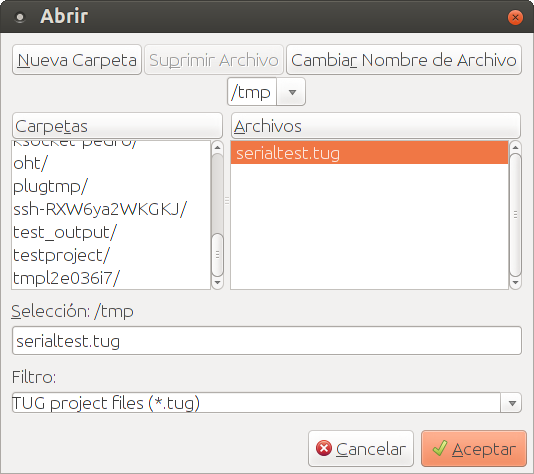
\includegraphics[width=.7\textwidth]{images/tug_load2.png}
\vspace{3ex}
\newpage

%
%%% 
%%
\item {\bf Save a TUG project.}\\
%
  Click 
\includegraphics[width=.05\textwidth]{images/menu_icon.png}
  to deploy the pop-up menu and select \field{Save TUG project}.\\
%
  Select a {\tt *.tug} file or write a new name for the project. Click
  \field{OK}. Data will be restored into TUG Wizard fields.


\vspace{1ex}

\includegraphics[width=.5\textwidth]{images/tug_save.png}

\vspace{1ex}
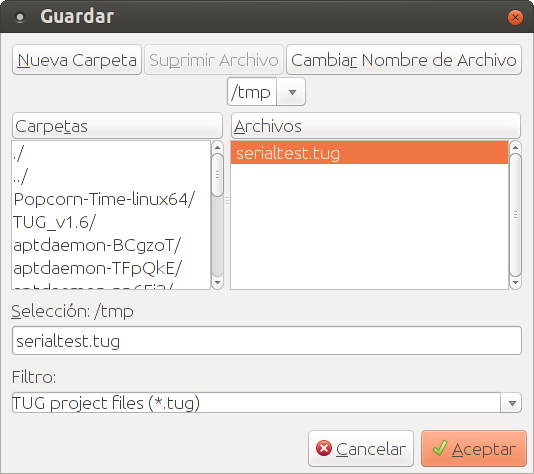
\includegraphics[width=.7\textwidth]{images/tug_save2.png}
\vspace{3ex}



\end{enumerate}
\newpage




%%% Local variables:
%%% mode: latex
%%% TeX-master: "README.tex"
%%% ispell-local-dictionary: "american"
%%% coding: utf-8
%%% fill-column: 75
%%% TeX-parse-self: t
%%% TeX-auto-save: t
%%% End:
